\chapter{基于多层空间和通道注意力网络的图像描述语句生成方法}

视觉注意力机制已经被广泛地运用在多模态任务中,如描述语句生成、视觉问答等。现有的注意力机制都是空间注意力机制,即只对卷积神经网络的最后一个特征图(feature map)在空间维度上进行加权。但是,卷积神经网络除了空间维度以外,还有通道维度,以及多层的特性。因此,目前的空间注意力机制并没有充分利用卷积神经网络的特性。在本章,我们提出一种全新的卷积神经网络:空间和通道注意力卷积神经网络(Spatial and Channel-wise Attention in CNN, SCA-CNN)。对于图像描述语句生成任务,在生成每个单词的过程中,SCA-CNN可以动态地融合不同空间位置、不同通道、不同层之间特征的内在联系。我们在图像描述语句生成的三个标准数据集上(Flickr8K, Flickr30K和MSCOCO)对模型SCA-CNN进行评估,大量的对比实验结果都表明我们提出的空间和通道注意力机制(SCA-CNN)可以显著地提升图像描述语句生成的性能。


\section{问题描述}

视觉注意力机制已经被广泛地证明可以用来提升多模态任务性能,如图像或视频的描述语句生成~\cite{xu2015show,yao2015describing}、视觉问答~\cite{chen2016abc,yang2016stacked,xu2016ask}等。注意力机制主要是基于一个合理的设想:人类在做图像描述语句生成任务时,人类不是一次性记住整个图像,而是在生成语句的过程中不断地去调整关注的区域~\cite{corbetta2002control}。具体来说,与之前工作直接将整个图像编码成一个固定的向量表达不同,注意力机制让模型在语句生成过程中不断的调整图像表达,从而生成更加丰富和准确的描述语句。因此,注意力机制也可以看成是一种动态的特征调节机制~\cite{mnih2014recurrent,stollenga2014deep}。

目前主要的图像特征都是通过卷积神经网络进行编码~\cite{he2016deep,simonyan2015very}。给定一个大小为$W\times H\times 3$的彩色图像,通常卷积层用一个通道数为$C$的卷积核进行卷积,得到一个大小为$W'\times H'\times C$的特征图,然后这个特征图又输入到后续的网络结构中。三维的特征图中每个通道对应的是卷积核通道对应的响应。其中,卷积核也可以看成是一种模式检测器:底层的卷积核倾向于检测一些底层的视觉特征(如:边、角等),高层的卷积核倾向于检测一些高层的语义特征(如:物体等)~\cite{zeiler2014visualizing}。通过叠加多个卷积层,卷积神经网络实现对图像的多层语义特征提取。因此,卷积神经网络的图像特征本质上有三种维度:空间维度、通道维度、和层级维度。然后,目前所有的工作都只考了空间维度~\cite{xu2015show},即:只利用语句信息对卷积神经网络的最后一个特征图在空间维度上进行加权。


\begin{figure}[htbp]
    \centering
    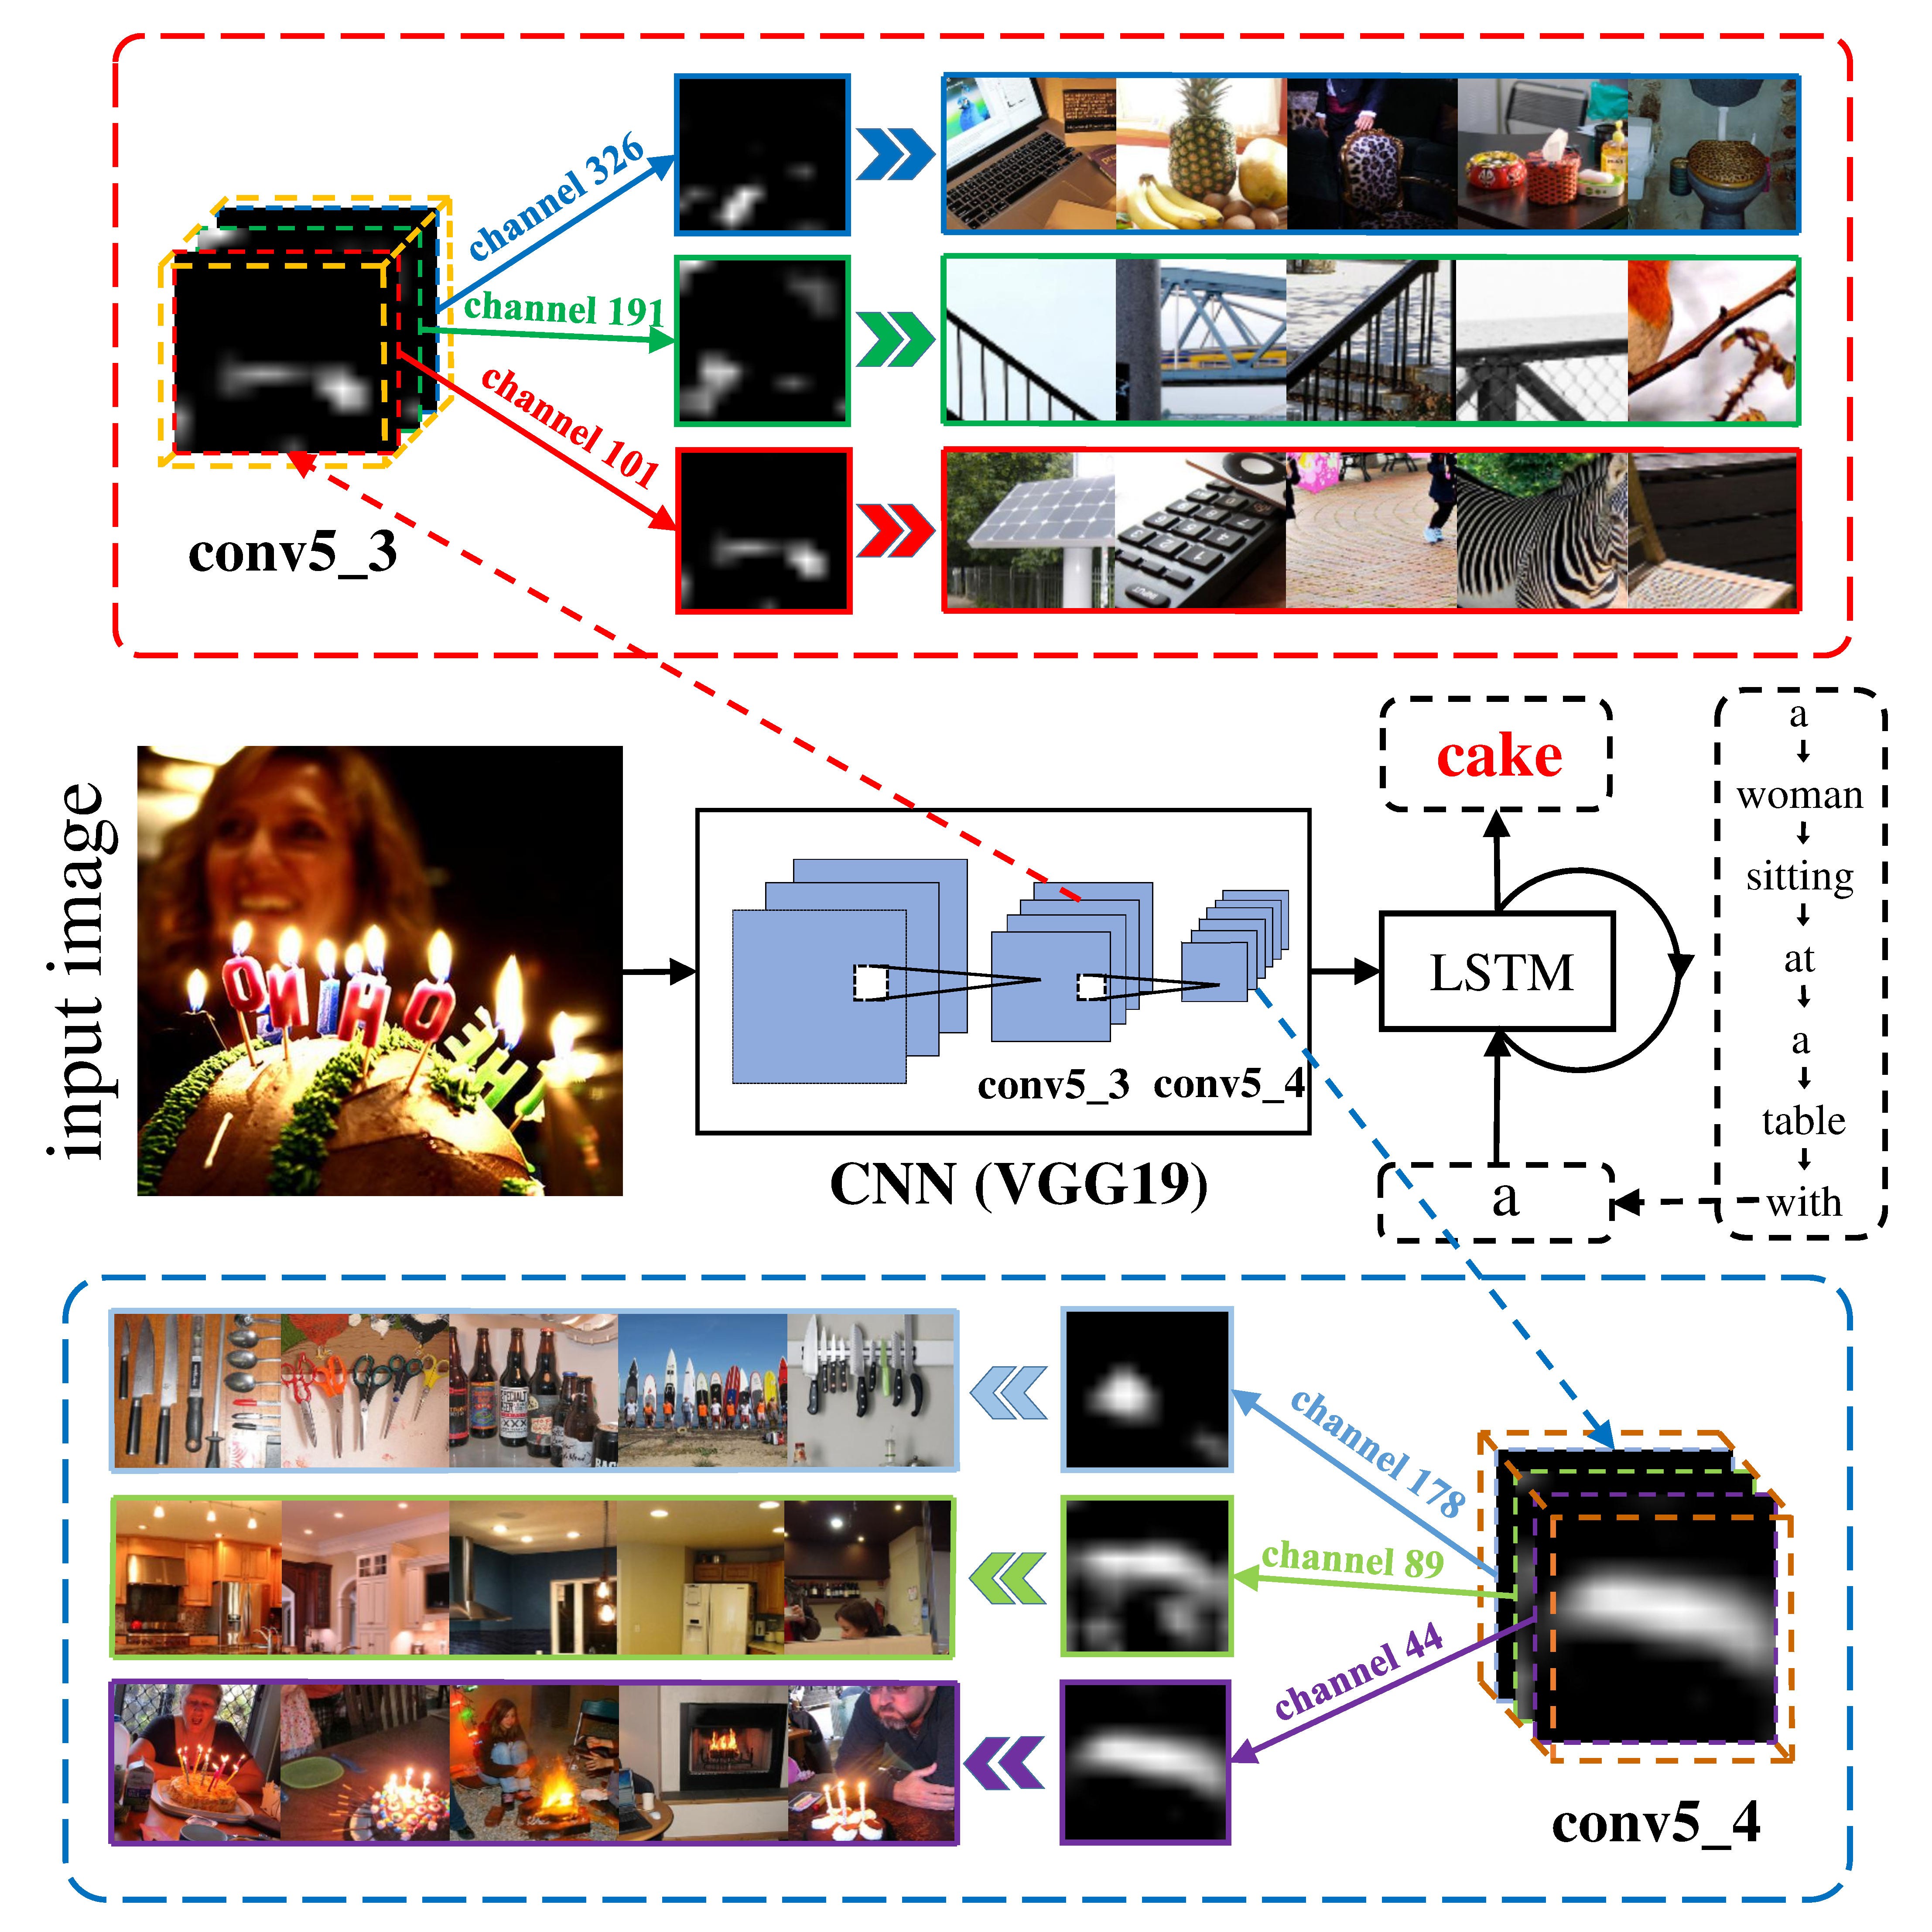
\includegraphics[width=0.8\linewidth]{chapter5/res/motivation.pdf}
    \caption{VGG19网络中$conv5\_4$层和$conv5\_3$层的通道注意力机制示例图}
    \label{ch5:fig:motivation}
\end{figure}



在本章,我们在基于注意力机制的图像描述语句生成模型中,将充分利用卷积神经网络的图像特征的三个维度。具体来说,我们提出了一种全新的网络结构:空间和通道注意力卷积神经网络(SCA-CNN),对多个卷积层的所有元素都进行加权。如图~\ref{ch5:fig:motivation}所示,特征图的每一个通道本质上可以认为是一种特定属性或者物体检测器的响应结果,即通道注意力可以看成是基于生成语句对不同的属性特征进行选择。例如,当模型要预测单词“cake”时,通道注意力会对部分属性特征赋予更大的权重,如火、光、蜡烛形状等。另外,由于每个卷积层都是底层卷积的输出结果,因此,可以对多个不同的卷积层都使用空间和通道注意力机制,让低层特征(如图~\ref{ch5:fig:motivation}中$conv5\_3$)关注更加底层的属性特征。

我们在三个标准的数据集(Flickr8K、Flickr30K和MSCOCO)对SCA-CNN的性能进行评估。SCA-CNN可以比现有的空间注意力模型~\cite{xu2015show}在评价指标BLEU4上提升4.8\%。总而言之,我们提出了一种全新的卷积神经网络结构,对网络特征层在空间上、通道上、和层级上三个维度进行注意力加权。SCA-CNN模型是一种通用的结构,可以运用在任意的网络结构和网络层上,如VGG~\cite{simonyan2015very}和ResNet~\cite{he2016deep}。SCA-CNN也帮助我们更好的理解卷积神经网络特征在描述语句生成过程中的变化过程。



\section{空间和通道注意力机制}

\subsection{概述}
我们采用流行的编码-解码框架对图像生成描述语句,即先用编码器(卷积神经网络)将图像编码成一个向量表达,然后使用解码器(递归神经网络)将图像视觉表达解码成描述语句。如图~\ref{ch5:fig:architecture}所示,SCA-CNN利用语句信息对不同层级的特征进行空间和通道注意力加权。

假设模型在生成第$t$个单词,此时LSTM的隐含状态为$\mathbf{h}_{t-1}\in\mathbb{R}^d$,其中$d$是隐含状态的维度。对于第$l$层的特征,SCA-CNN根据$\mathbf{h}_{t-1}$和目前的卷积特征$\mathbf{V}^l$,可以得到新的卷积特征$\mathbf{X}^l$:
\begin{equation} \label{ch5:eq:eq_1}
\begin{split}
\mathbf{V}^l &= \textrm{CNN}\left(\mathbf{X}^{l-1}\right),\\
\gamma^l &= \Phi\left(\mathbf{h}_{t-1},\mathbf{V}^l\right),\\
\mathbf{X}^l &= f\left(\mathbf{V}^{l},\gamma^{l}\right).
\end{split}
\end{equation}
其中,$\Phi(\cdot)$是空间和通道注意力函数,$\mathbf{V}^l$是上一个卷积层的输出$mathbf{X}^{l-1}$之后再接卷积层或池化层~\cite{simonyan2015very,he2016deep},$f(\cdot)$是线性加权函数。当卷积特征达到最后一层(第$L$层)时,我们使用$\mathbf{X}^L$来生成第$t$个单词:
\begin{equation}
\begin{split}
\mathbf{h}_t &= \textrm{LSTM}\left(\mathbf{h}_{t-1},\mathbf{X}^L,y_{t-1}\right),\\
y_t & \sim p_t = \textrm{softmax} \left(\mathbf{h}_t, y_{t-1} \right).
\end{split}
\end{equation}
其中,$p_t \in \mathbb{R}^{|\mathcal{D}|}$是字典中所有单词的预测概率,$\mathcal{D}$是字典包含训练集语句中出现的所有单词。

如果注意力参数$\gamma^l$与特征$\mathbf{V}^l$或$\mathbf{X}^l$同时的尺寸($W^l\times H^l\times C^l$),其计算量大小为$\mathcal{O}(W^lH^lC^lk)$,其中$k$是卷积网络特征$\mathbf{V}^l$和LSTM的隐含状态$\mathbf{h}_{t-1}$映射到同一空间中的维度大小。在特征图尺寸非常大时,对GPU的需求比较大。因此,我们提出将三维的$\gamma^l$分解成空间注意力参数$\alpha^l$和通道注意力参数$\beta^l$:
\begin{eqnarray}
\alpha^l &= & \Phi_s \left(\mathbf{h}_{t-1},\mathbf{V}^l\right),  \label{ch5:eq:eq_3} \\
\beta^l &= & \Phi_c \left(\mathbf{h}_{t-1},\mathbf{V}^l\right). \label{ch5:eq:eq_4}
\end{eqnarray}
其中$\Phi_c$和$\Phi_s$分别表示通道注意力模型和空间注意力模型。这种简化将极大地减小计算空间到$\mathcal{O}(C^lk+W^lH^lk)$。

\begin{figure}[tbp]
    \centering
    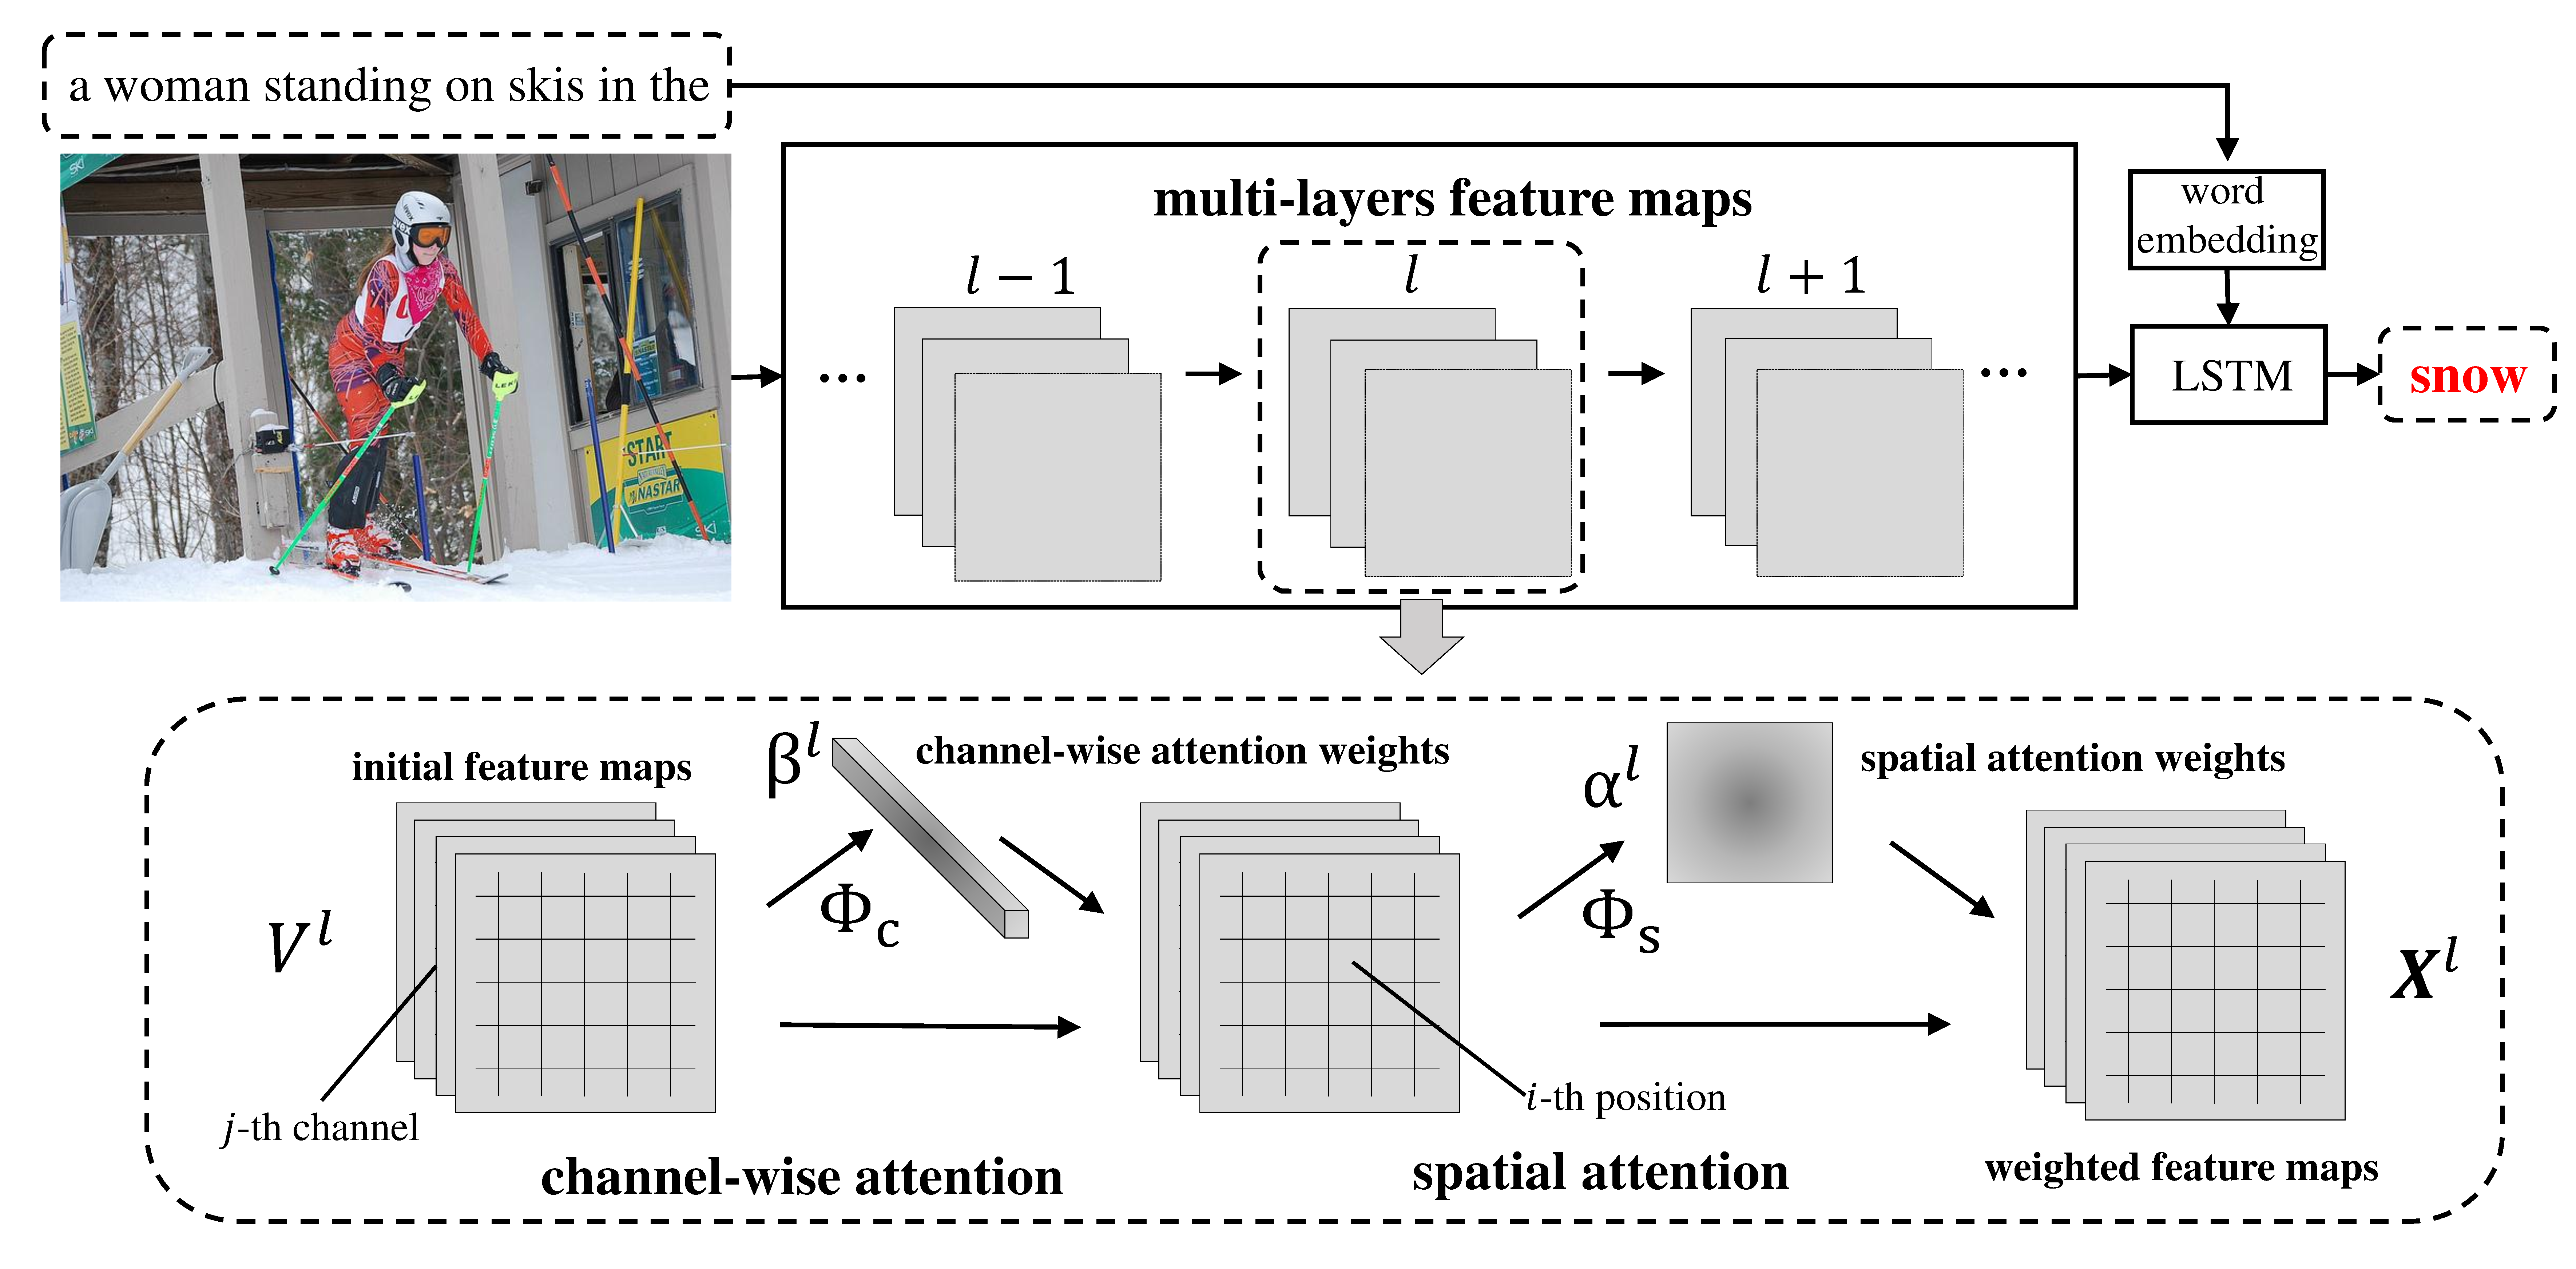
\includegraphics[width=\linewidth]{chapter5/res/architecture.pdf}
    \caption{空间和通道注意力卷积神经网络流程图}
    \label{ch5:fig:architecture}
\end{figure}


\subsection{空间注意力机制}
通常,每个单词只与图像中的部分区域有关,如图~\ref{ch5:fig:motivation},当预测单词“cake”时,只有包含蛋糕的图像区域对于“cake”的预测有用。因此,在生成每个单词时,都用同一个全局图像特征容易使模型陷入局部最优解。空间注意力机制就是对不同的图像区域(空间上)赋予不同的权重。为了不失一般性,我们省略层数上角标$l$。我们先将视觉特征$\mathbf{V}$变形成$\mathbf{V}  = \left[\mathbf{v}_1, \mathbf{v}_2, ..., \mathbf{v}_m
\right]$,其中$\mathbf{v}_i\in\mathbb{R}^C$,$m=W\cdot H$,$\mathbf{v}_i\in\mathbb{R}^C$可以看成是第$i$个位置的图像特征。给定上一个时刻的LSTM的隐含状态$\mathbf{h}_{t-1}$,我们使用单层神经网络生成空间注意力权重$\alpha$:
\begin{equation} \label{ch5:eq:eq_5}
\begin{split}
\mathbf{a} & = \tanh \left( \left( \mathbf{W}_s \mathbf{V} + b_s \right) \oplus \mathbf{W}_{hs}\mathbf{h}_{t-1}\right), \\
\alpha & = \textrm{softmax} \left( \mathbf{W}_i \mathbf{a} + b_i \right).
\end{split}
\end{equation}
其中,$\mathbf{W}_s \in \mathbb{R}^{k \times C}$、$\mathbf{W}_{hs} \in \mathbb{R}^{k \times d}$、$\mathbf{W}_i \in \mathbb{R}^k$都是需要学习的映射矩阵,这些矩阵分别将视觉特征、隐含状态映射到同一个维度。$\oplus$表示矩阵和向量相加,即对矩阵中的每一个列向量都加上该向量。$b_s \in \mathbb{R}^k, b_i \in \mathbb{R}^1$是模型中可学习的偏置。


\subsection{通道注意力机制}
从公式~\ref{ch5:eq:eq_3}中可以看出,空间注意力机制需要使用视觉特征$\mathbf{V}$计算空间注意力参数,我们也同时可以使用通道注意力机制对$\mathbf{V}$进行通道注意力加权。因为卷积神经网络的特征图的每一个通道本质上可以认为是一种特定属性或者物体检测器的响应结果,因此,对特征图使用通道注意力机制可以看成是对不同的语义特征进行删选的过程。

对于通道注意力机制,我们先将特征图$\mathbf{V}$转变为$\mathbf{U}$,其中$\mathbf{U} = [\mathbf{u}_1, \mathbf{u}_2, ..., \mathbf{u}_C]$、$\mathbf{u}_i \in \mathbb{R}^{W \times H}$表示特征图$\mathbf{V}$的第$i$个通道,$C$是总的通道数。然后我们对每个通道使用平均池化,得到通道特征$\mathbf{v}$:
\begin{equation}
\mathbf{v} = \left[v_1, v_2, ..., v_C \right], \mathbf{v} \in \mathbb{R}^{C},
\end{equation}
其中标量$v_i$是向量$\mathbf{u}_i$的平均,表示第$i$个通道的特征。于是,通道注意力模型$\Phi_c$可以定义为:
\begin{equation} \label{ch5:eq:eq_7}
\begin{split}
\mathbf{b} & = \tanh \left(\left(\mathbf{W}_c \otimes \mathbf{v} + b_c \right) \oplus \mathbf{W}_{hc}\mathbf{h}_{t-1} \right), \\
\beta & = \textrm{softmax} \left(\mathbf{W'}_i \mathbf{b} + {b'}_i \right).
\end{split}
\end{equation}
其中$\mathbf{W}_c \in \mathbb{R}^k$、$\mathbf{W}_{hc} \in \mathbb{R}^{k \times d}$和$\mathbf{W'}_i \in \mathbb{R}^k$是需要学习的映射矩阵,$\otimes$表示向量间的外积,$b_c \in \mathbb{R}^k, {b'}_i \in \mathbb{R}^1$是模型可学习的偏置。

根据空间注意力模型和通道注意力模型的顺序,共有两种可能的组合结果:

\textbf{通道-空间模型(Channel-Spatial)}:第一类是先使用通道注意力机制再使用空间注意力机制。对于这类,如图~\ref{ch5:fig:architecture}所示,给定一个初始的视觉特征图$\mathbf{V}$,我们先使用通道注意力模型$\Phi_c$得到通道注意力权重$\beta$,然后利用$\beta$对$\mathbf{V}$进行线性加权。之后,我们将加权的特征图输入到空间注意力模型$\Phi_s$得到空间注意力权重$\alpha$。在得到注意力权重$\alpha$和$\beta$之和,我们可以得到最终的特征图$\mathbf{X}$:
\begin{equation} \label{ch5:eq:eq_8}
\begin{split}
\beta &= \Phi_c \left(\mathbf{h}_{t-1},\mathbf{V} \right), \\
\alpha &= \Phi_s \left(\mathbf{h}_{t-1}, f_c \left(\mathbf{V}, \beta \right) \right), \\
\mathbf{X} &= f \left(\mathbf{V}, \alpha, \beta \right).
\end{split}
\end{equation}
其中,$f_c(\cdot)$表示特征图通道与通道注意力权重在通道维度上进行乘积。


\textbf{空间-通道模型(Spatial-Channel)}:第二类是先使用空间注意力机制再使用通道注意力机制。对于这类,给定一个初始的视觉特征图$\mathbf{V}$,我们先使用空间注意力模型$\Phi_s$得到空间注意力权重$\alpha$。通过$\alpha$、线性函数$f_s(\cdot)$和通道注意力模型$\Phi_c$,我们可以得到最终的特征图$\mathbf{X}$:
\begin{equation} \label{ch5:eq:eq_9}
\begin{split}
\alpha &= \Phi_s \left(\mathbf{h}_{t-1}, \mathbf{V} \right), \\
\beta &= \Phi_c \left(\mathbf{h}_{t-1}, f_s \left(\mathbf{V}, \alpha \right) \right), \\
\mathbf{X} &= f \left(\mathbf{V}, \alpha, \beta \right).
\end{split}
\end{equation}
其中,$f_s(\cdot)$表示特征图空间不同区域特征与空间注意力权重进行乘积。



\section{实验设置与性能对比}
\subsection{图像描述语句生成数据集}
\noindent\textbf{Flickr8k}~\cite{hodosh2013framing}:它一共包含8000张图像。按照官方划分,我们将其中6000张图像作为训练集,1000张图像为验证集,以及1000张图像为测试集。

\noindent\textbf{Flickr30k}~\cite{young2014image}: 它一共包含31000张图像。因为这个数据集缺少官方划分,我们采用与之前工作~\cite{karpathy2015deep}同样的划分。在这种划分中,29000张图像作为训练集,1000张图像为验证集,以及1000张图像为测试集。

\noindent\textbf{MSCOCO}~\cite{lin2014microsoft}:根据该数据集的官方划分,训练集包含82783张图像,验证集包含40504张图像,以及测试集包含40775张图像。对于官方测试集,由于所有的图像都没有公布其中的人工标注信息,我们同样参考之前的工作~\cite{karpathy2015deep}将官方验证集划分为验证集和测试集两部分,其中验证集和测试集各包含5000张图像。


\subsection{评价指标}
\noindent\textbf{BLEU}~\cite{papineni2002bleu} (B@1, B@2, B@3, B@4):

\noindent\textbf{METEOR}~\cite{banerjee2005meteor} (MT):

\noindent\textbf{CIDEr}~\cite{vedantam2015cider} (CD):

\noindent\textbf{ROUGE-L}~\cite{lin2002manual} (RG):


对于所有的四种评价指标来说,他们都是通过比较生成语句中的n元词组在人工标注的语句中出现的频率。所有的评价指标都是采用MSCOCO官方的测评工具\footnote{https://github/tylin/coco-caption.}。



\subsection{实验设定}
对于图像编码部分,我们采用两种流行的卷积神经网络:VGG-19~\cite{simonyan2015very}和ResNet-152~\cite{he2016deep}。对于文本解码部分,我们使用LSTM~\cite{hochreiter1997long}来生成描述语句中的单词。单词编码的维度和LSTM的隐含状态的维度分别设定为100和1000。用于计算注意力权重的共同空间维度设置为512。对于Flickr8k数据集,batch size设置为16;对于Flickr30k和MSCOCO,batch size设置为64。为了避免过拟合,我们采用dropout和early stopping。我们整个模型采用端到端的训练方式,用优化算法Adadelta~\cite{zeiler2012adadelta}进行参数优化。整个语句的生成过程将会终止当模型刚好预测一个特定的“END”字符或者达到了预先设定的句子最长的长度。在测试阶段,我们采用BeamSearch~\cite{vinyals2015show}的方法,在每个时刻选择5个句子作为候选答案。


\subsection{通道注意力机制的性能分析}

\textbf{实验设定}:本小节主要探讨通道注意力机制对现有空间注意力模型的影响。我们总共比较了五种实验设定:(1)\textbf{Spatial}:它是一个空间注意力模型,对卷积网络最后一层特征图先计算空间注意力权重,然后对最后一层特征图的不同空间区域特征进行加权。对于VGG19和ResNet152网络,最后一层分别为$conv5\_4$和$res5c$。对最后一层进行加权之后,我们将加权后的特征图输入的原本的网络结构中。对于VGG19网络而言,$conv5\_4$层之后还有两个全连接层;对于ResNet152网络而言,$res5c$层之后是一个平均池化层。(2)\textbf{Channel}:它是一个通道注意力模型,和空间注意力模型Spatial基本相同,除了将空间注意力模型(公式~\eqref{ch5:eq:eq_3})替换成通道注意力模型(公式~\eqref{ch5:eq:eq_4})。(3)\textbf{Channel-Spatial}:第一种融合方式,先执行通道注意力模型,再执行空间注意力模型(公式~\eqref{ch5:eq:eq_8})。(4)\textbf{Spatial-Channel}:第二种融合方法,先执行空间注意力模型,再执行通道注意力模型(公式~\eqref{ch5:eq:eq_9})。(5)\textbf{HAT}:它是Xu等人~\cite{xu2015show}提出的“硬”注意力模型(Hard-ATtention, HAT)。HAT模型和Spatial模型一样,属于空间注意力模型。相比于Spatial模型,主要有两个区别:第一个是注意力权重和特征图的融合方式,第二个是是否将加权的特征图输入到候选的网络结构中。所有的实验结果都展示在表~\ref{ch5:tab:Q1}中。

%%%%%%%%%%%%%%%%%%%%%% Q1 %%%%%%%%%%%%%%%%%%%%%%%%%%%%%%%
\begin{table}[htbp]
\centering
\scalebox{0.75}{
\begin{tabular}{|l| l |l| c c c c|}
\hline
 Dataset & Network &Method & B@4 & MT & RG & CD\\
\hline
\multirow{10}{*}{Flickr8k} & \multirow{5}{*}{VGG} & Spatial & 23.0 & 21.0 & 49.1 & \textbf{60.6} \\
&  & HAT & 21.3 & 20.3 & --- & --- \\
&  & Channel & 22.6 & 20.3 & 48.7 & 58.7 \\
& & Spatial-Channel &22.6 & 20.9 & 48.7 & \textbf{60.6}\\
& & Channel-Spatial & \textbf{23.5} & \textbf{21.1} & \textbf{49.2} & 60.3\\
\cline{2-7}
& \multirow{5}{*}{ResNet} & Spatial & 20.5 & 19.6 & 47.4 & 49.9 \\
&  & HAT & 21.7 & 20.1 & 48.4 & 55.5 \\
&  & Channel & 24.4 & 21.5 & 50.0 & 65.5 \\
& & Spatial-Channel &24.8 & \textbf{22.2} & 50.5& 65.1\\
& & Channel-Spatial & \textbf{25.7} & 22.1& \textbf{50.9} & \textbf{66.5}\\
\hline
\multirow{10}{*}{Flickr30k} & \multirow{5}{*}{VGG} & Spatial & \textbf{21.1} & 18.4 & 43.1 & \textbf{39.5} \\
&  & HAT & 19.9 & \textbf{18.5} &  --- & --- \\
&  & Channel & 20.1 & 18.0 & 42.7 & 38.0 \\
& & Spatial-Channel & 20.8 & 17.8&42.9 & 38.2\\
& & Channel-Spatial & 21.0 & 18.0& \textbf{43.3} & 38.5\\
\cline{2-7}
& \multirow{5}{*}{ResNet} & Spatial & 20.5 & 17.4 & 42.8 & 35.3 \\
&  & HAT & 20.1 & 17.8 & 42.9 & 36.3 \\
&  & Channel & 21.5 & 18.4 & 43.8 & 42.2 \\
& & Spatial-Channel &21.9 & 18.5 & 44.0& \textbf{43.1}\\
& & Channel-Spatial & \textbf{22.1} & \textbf{19.0} & \textbf{44.6} & 42.5 \\
\hline
\multirow{10}{*}{MS COCO} & \multirow{5}{*}{VGG} & Spatial & \textbf{28.2} & 23.3 & \textbf{51.0} & \textbf{85.7} \\
&  & HAT & 25.0 & 23.0 & --- & --- \\
&  & Channel & 27.3 & 22.7 & 50.1 & 83.4 \\
& & Spatial-Channel &28.0 &23.0 & 50.6& 84.9\\
& & Channel-Spatial & 28.1 & \textbf{23.5} & 50.9& 84.7\\
\cline{2-7}
& \multirow{5}{*}{ResNet} & Spatial & 28.3 & 23.1 & 51.2 & 84.0 \\
&  & HAT & 28.4 & 23.2 & 51.2 & 84.9 \\
&  & Channel & 29.5 & 23.7 & 51.8 & 91.0 \\
& & Spatial-Channel &29.8 &23.9 & 52.0& 91.2\\
& & Channel-Spatial & \textbf{30.4} & \textbf{24.5} & \textbf{52.5} & \textbf{91.7}\\
\hline
\end{tabular}}
\caption{VGG-19网络和ResNet-152网络单层注意力机制的性能对比} 
\label{ch5:tab:Q1}
\end{table}
%%%%%%%%%%%%%%%%%%%%%%%%%%%%%%%%%%%%%%%%%%%%%%%%%%%%%%%%%


\textbf{实验结果}:从表~\ref{ch5:tab:Q1}中可以看出,(1)对于VGG19网络而言,Spatail模型的结果比HAT的好;但对于ResNet152网络,实验结果相反。这主要的原因在于VGG19网络中有全连接层,可以保持空间语义信息,而ResNet152网络中只有只有平均池化层,将会破坏原有的空间语义信息。(2)相比于VGG19网络,Channel模型在ResNet152中可以显著提升性能(与Spatial模型相比)。这主要的原因在于ResNet152的最后一个卷积特征图拥有更多的通道数(如:ResNet152有2048个通道相比于VGG19有512个通道)。(3)在ResNet152网络中,相比于Spatial模型,Channel-Spatial和Spatial-Channel都能显著提升性能。这说明通道注意力机制在特征图通道数足够大时能显著提升性能。(4)在VGG19和ResNet152网络中,Channel-Spatial和Spaital-Channel两个模型的效果都非常接近,其中Channel-Spatial稍微高一点,在之后的实验中,我们使用Channel-Spatial作为融合方式。


%%%%%%%%%%%%%%%%%%%%%% Q2_1 %%%%%%%%%%%%%%%%%%%%%%%%%%
\begin{table}[htbp]
\centering
\scalebox{0.8}{
\begin{tabular}{|l| l |l| c c c c|}
\hline
 Dataset & Network &Method & B@4 & MT & RG & CD\\
\hline
\multirow{6}{*}{Flickr8k} & \multirow{3}{*}{VGG} & 1-layer & \textbf{23.0} & 21.0 & \textbf{49.1} & \textbf{60.6} \\
&  & 2-layer & 22.8 & \textbf{21.2} & 49.0 & 60.4 \\
&  & 3-layer & 21.6 & 20.9 & 48.4 & 54.5 \\
\cline{2-7}
& \multirow{3}{*}{ResNet} & 1-layer & 20.5 & 19.6 & 47.4 & 49.9 \\
&  & 2-layer & 22.9 & 21.2 & 48.8 & 58.8 \\
&  & 3-layer & \textbf{23.9} & \textbf{21.3} & \textbf{49.7} & \textbf{61.7} \\
\hline
\multirow{6}{*}{Flickr30k} & \multirow{3}{*}{VGG} & 1-layer & 21.1 & 18.4 & 43.1 & \textbf{39.5} \\
&  & 2-layer & \textbf{21.9} & \textbf{18.5} & \textbf{44.3} & \textbf{39.5} \\
&  & 3-layer & 20.8 & 18.0 & 43.0 & 38.5 \\  %%%%%%%%%
\cline{2-7}
& \multirow{3}{*}{ResNet} & 1-layer & 20.5 & 17.4 & 42.8 & 35.3 \\
&  & 2-layer & 20.6 & 18.6 & 43.2 & 39.7 \\
&  & 3-layer & \textbf{21.0} & \textbf{19.2} & \textbf{43.4} & \textbf{43.5} \\
\hline
\multirow{6}{*}{MS COCO} & \multirow{3}{*}{VGG} & 1-layer & 28.2 & 23.3 & 51.0 & 85.7 \\
&  & 2-layer & \textbf{29.0} & \textbf{23.6} & \textbf{51.4} & \textbf{87.4}\\
&  & 3-layer & 27.4 & 22.9 & 50.4 & 80.8 \\
\cline{2-7}
& \multirow{3}{*}{ResNet} & 1-layer & 28.3 & 23.1 & 51.2 & 84.0 \\
&  & 2-layer & \textbf{29.7} & 24.1 & \textbf{52.2} & \textbf{91.1} \\
&  & 3-layer & 29.6 & \textbf{24.2} & 52.1 & 90.3 \\
\hline
\end{tabular}}
\caption{空间注意力模型在VGG-19网络和ResNet-152网络下不同层的性能对比} 
\label{ch5:tab:Q2_1}
\end{table}
%%%%%%%%%%%%%%%%%%%%%%%%%%%%%%%%%%%%%%%%%%%%%%%%%%%%%


\subsection{多层注意力机制的性能分析}

\textbf{实验设定}:本小节主要探讨对不同的卷积层使用空间注意力机制或通道注意力机制对模型性能的影响。我们分别对Spatial模型和Channel-Spatial模型进行了不同层数的实验:一层(1-layer)、两层(2-layer)、和三层(3-layer)。对于VGG19网络,这三层分别表示:$conv5\_4$、$conv5\_3$、$conv5\_2$;对于ResNet152网络,这三层分别表示$res5c$、$res5c\_branch2b$、$res5c\_branch2a$。在我们的实验中,对于更多的层,我们先使用已训练好的参数作为初始化,将极大地减小训练时间和收敛速度。


%%%%%%%%%%%%%%%%%%%%% Q2_2 %%%%%%%%%%%%%%%%%%%%%%%%%
\begin{table}[htbp]
\centering
\scalebox{0.8}{
\begin{tabular}{|l| l |l| c c c c|}
\hline
 Dataset & Network &Method & B@4 & MT & RG & CD\\
\hline
\multirow{6}{*}{Flickr8k} & \multirow{3}{*}{VGG} & 1-layer & \textbf{23.5} & 21.1 & 49.2 & 60.3 \\
&  & 2-layers & 22.8 & \textbf{21.6} & \textbf{49.5} & 62.1 \\
&  & 3-layers & 22.7 & 21.3 & 49.3 & \textbf{62.3} \\
\cline{2-7}
& \multirow{3}{*}{ResNet} & 1-layer & 25.7 & 22.1 & 50.9 & 66.5 \\
&  & 2-layers & \textbf{25.8} & 22.4 & \textbf{51.3} & 67.1 \\
&  & 3-layers & 25.3 & \textbf{22.9} & 51.2 & \textbf{67.5} \\
\hline
\multirow{6}{*}{Flickr30k} & \multirow{3}{*}{VGG} & 1-layer & 21.0 & 18.0 & 43.3 & 38.5 \\
&  & 2-layers & \textbf{21.8} & \textbf{18.8} & \textbf{43.7} & \textbf{41.4} \\
&  & 3-layers & 20.7 & 18.3 & 43.6 & 39.2 \\
\cline{2-7}
& \multirow{3}{*}{ResNet} & 1-layer & 22.1 & 19.0 & 44.6 & 42.5 \\
&  & 2-layers & \textbf{22.3} & \textbf{19.5} & \textbf{44.9} & \textbf{44.7} \\
&  & 3-layers & 22.0 & 19.2 & 44.7 & 42.8 \\        %%
\hline
\multirow{6}{*}{MS COCO} & \multirow{3}{*}{VGG} & 1-layer & 28.1 & 23.5 & 50.9 & 84.7 \\
&  & 2-layers & \textbf{29.8} & \textbf{24.2} & \textbf{51.9} & \textbf{89.7} \\
&  & 3-layers & 29.4 & 24.0 & 51.7 & 88.4 \\    %%
\cline{2-7}
& \multirow{3}{*}{ResNet} & 1-layer & 30.4 & 24.5 & 52.5 & 91.7 \\
&  & 2-layers & \textbf{31.1} & \textbf{25.0} & \textbf{53.1} & \textbf{95.2} \\
&  & 3-layers & 30.9 & 24.8 & 53.0 & 94.7 \\   %%
\hline
\end{tabular}}
\caption{空间和通道注意力模型在VGG-19网络和ResNet-152网络下不同层的性能对比} 
\label{ch5:tab:Q2_2}
\end{table}
%%%%%%%%%%%%%%%%%%%%%%%%%%%%%%%%%%%%%%%%%%%%%%%%%%%%%%%%%

\textbf{实验结果}:从表~\ref{ch5:tab:Q2_1}和表~\ref{ch5:tab:Q2_2}可以看出:(1)在绝大多数的实验设定中,模型都可以通过在更多的卷积层上使用注意力机制来提升实验结果。这主要是因为在多层特征上使用注意力机制可以帮助模型在不同的层次的语义特征上进行关注。(2)在太多的卷积层上使用注意力机制也容易造成过拟合。例如:当注意力机制改变的层数增加时,Flickr8K更容易造成性能下降(Fickr8K有6000张训练图像,而MSCOCO有82783张训练图像)。



\subsection{空间和通道注意力卷积神经网络的性能比较}

\textbf{实验设定}:我们与目前效果最好的图像描述语句算法进行对比,这些方法主要可以分为三类:(1)Deep VS~\cite{karpathy2015deep}、NIC~\cite{vinyals2015show}、m-RNN~\cite{mao2015deep}:这些都是端到端的编码-解码框架,模型中没有包含注意力机制。(2)SAT~\cite{xu2015show}和HAT~\cite{xu2015show}是空间注意力模型。其中SAT(Soft-ATtention)是在每步生成单词的过程中对所有的空间区域进行线性加权,而HAT(Hard-ATtention)是在每步生成单词的过程中对所有的区域只采样其中一个特征。(3)gLSTM~\cite{jia2015guiding}和ATT~\cite{you2016image}是属性注意力机制。其中gLSTM使用图像和生成的描述语句作为全局的属性信息,ATT使用图像额外检测的属性作为属性信息。表~\ref{ch5:tab:sota}的结果“ours(V)”和“ours(R)”分别表示VGG19和ResNet152网络中两层Channel-Spatial模型。另外,我们还将模型上传到MSCOCO在线服务器对官方测试集进行预测,结果展示在表~\ref{ch5:tab:server}中。

%%%%%%%%%%%%%%%%%%%%%%% Q3 %%%%%%%%%%%%%%%%%%%%%%%%%%%
\begin{table*}[htbp]
\centering
\scalebox{0.8}{
\begin{tabular}{ |l | c c c c  | c c c c | c c c c|}
\hline
\multirow{2}{*}{Model} & \multicolumn{4}{c|}{Flickr8k} & \multicolumn{4}{c|}{Flickr30k} & \multicolumn{4}{c|}{MS COCO} \\
\cline{2-13}
& B@2 & B@3 & B@4 & MT & B@2 & B@3 & B@4 & MT & B@2 & B@3 & B@4 & MT \\
\hline
Deep VS & 38.3 & 24.5 & 16.0 & -- &  36.9 & 24.0 & 15.7 & --  & 45.0 & 32.1 & 23.0 & 19.5 \\
NIC & 41.0 & 27.0 & -- & -- & 42.3 & 27.7 & 18.3  & -- & 46.1 & 32.9 & 24.6 & -- \\
m-RNN & -- & -- & -- & -- & 41.0 & 28.0 & 19.0 & -- & 49.0 & 35.0 & 25.0 & -- \\
SAT & 44.8 & 29.9 & 19.5 & 18.9 & 43.4 & 28.8 & 19.1 & 18.5 & 49.2 & 34.4 & 24.3 & 23.9 \\
HAT & 45.7 & 31.4 & 21.3 & 20.3 & 43.9 & 29.6 & 19.9 & 18.5 & 50.4 & 35.7 & 25.0 & 23.0 \\
gLSTM & 45.9 & 31.8 & 21.2 & 20.6 & 44.6 & 30.5 & 20.6 & 17.9 & 49.1 & 35.8 & 26.4 & 22.7 \\
ATT & -- & -- & -- & --  & 46.0 & 32.4 & \textbf{23.0} & 18.9 & 53.7 & 40.2 & 30.4 & 24.3  \\
\hline
ours(V) & 46.6 & 32.6 & 22.8 & 21.6 & 45.3 & 31.7 & 21.8 & 18.8 & 53.3 & 39.7 & 29.8 & 24.2\\
ours(R)  & \textbf{49.6} & \textbf{35.9} & \textbf{25.8} & \textbf{22.4} & \textbf{46.8} & \textbf{32.5} & 22.3 & \textbf{19.5} & \textbf{54.8} & \textbf{41.1} & \textbf{31.1} & \textbf{25.0}\\
\hline
\end{tabular}}
\caption{不同描述语句生成算法在数据集Flickr8k、Flickr30k和MSCOCO上的性能对比} 
\label{ch5:tab:sota}
\end{table*}
%%%%%%%%%%%%%%%%%%%%%%%%%%%%%%%%%%%%%%%%%%%%%%%%%%%%%%%%%

%%%%%%%%%%%%%%%%%%%%%%% sever %%%%%%%%%%%%%%%%%%%%%%%
\begin{table*}[htbp]
\centering
\scalebox{0.8}{
\begin{tabular}{ |l | c | c | c| c | c |c | c |c | c |c | c| c | c |c | }
\hline
\multirow{2}{*}{Model} & \multicolumn{2}{c|}{B@1} & \multicolumn{2}{c|}{B@2} & \multicolumn{2}{c|}{B@3} & \multicolumn{2}{c|}{B@4} &\multicolumn{2}{c|}{METEOR} & \multicolumn{2}{c|}{ROUGE-L} & \multicolumn{2}{c|}{CIDEr} \\
\cline{2-15}
& c5 & c40 & c5 & c40 & c5 & c40 & c5 & c40 & c5 & c40 & c5 & c40 & c5 & c40 \\
\hline
ours & 71.2 & 89.4 & 54.2& 80.2& 40.4& 69.1& 30.2& 57.9& 24.4 & 33.1 & 52.4 & 67.4& 91.2 & 92.1 \\
\hline
HAT  & 70.5& 88.1& 52.8& 77.9& 38.3 & 65.8 & 27.7 & 53.7 & 24.1 & 32.2& 51.6 &65.4 & 86.5 & 89.3\\
\hline
ATT & \textbf{73.1} & \textbf{90.0} & \textbf{56.5} & \textbf{81.5} & \textbf{42.4} & \textbf{70.9} & \textbf{31.6} & \textbf{59.9} &25.0 & \textbf{33.5} & 53.5& \textbf{68.2} & \textbf{95.3} & \textbf{95.8}   \\
\hline
NIC & 71.3 & 89.5 & 54.2& 80.2& 40.7& 69.4& 30.9& 58.7 & \textbf{25.4} & \textbf{34.6} & 53.0 & \textbf{68.2} & 94.3 & 94.6 \\
\hline
\end{tabular}}
\caption{不同图像描述语句生成算法在数据集MSCOCO的在线服务器上的性能对比} 
\label{ch5:tab:server}
\end{table*}
%%%%%%%%%%%%%%%%%%%%%%%%%%%%%%%%%%%%%%%%%%%%%%%%%%%%

\textbf{实验结果}:从表~\ref{ch5:tab:sota}和表~\ref{ch5:tab:server}中可以看出,SCA-CNN可以超过目前现有的模型,这是因为SCA-CNN分别考虑了卷积神经网络特征层的三个维度:空间、通道和层级,而其他的方法只考虑了其中一个维度。在MSCOCO在线服务器上,SCA-CNN性能比ATT和NIC低的主要原因来自两个方面:(1)ATT和NIC都是集成模型(ensemble model)的结果,而SCA-CNN是单个模型的结果。(2)它们使用更强的卷积神经网络对输入图像提取特征,如NIC使用Inception-V3网络~\cite{szegedy2016rethinking}而SCA-CNN只使用ResNet152网络。


\subsection{空间注意力和通道注意力权重的可视化}
如图~\ref{ch5:fig:visualization},我们还提供了一些SCA-CNN模型的注意力权重的在VGG19网络的可视化示例。其中“Layer-1”和“Layer-2”分别表示$conv5\_4$和$conv5\_3$层。每个示例包含三句描述语句:“Ours”(SCA-CNN)、“SAT”(Soft-ATtention)和“GT”(Ground Truth)。第二列的上部分是空间注意力权重,白色部分表示空间注意力权重较大,而灰色部分表示空间注意力权重较小。第二列下部分为所有通道权重的直方统计图。第三列的数字表示通道注意力权重最大的两个通道编号。后面的五张图像是数据集MSCOCO训练集中对同样通道编号响应最大的图像,其中红色框表示对应通道最强响应的感受野。为了简洁,我们只展示了预测语句中的其中一步。


\begin{figure}[htbp]
    \centering
    \includegraphics[width=\linewidth]{chapter5/res/visualization.pdf}
    \caption{空间注意力和通道注意力权重的可视化结果}
    \label{ch5:fig:visualization}
\end{figure}


\section{本章小结}

在本章,我们提出了一种全新的基于注意力机制的卷积神经网络(SCA-CNN)对图像生成描述语句。SCA-CNN充分利用了句卷积神经网络特征图的三个维度:空间、通道和层级;并且在图像描述语句生成任务达到了目前最好的性能。本章的贡献不仅仅是提出了一个更强的注意力机制,同时帮助理解在语句生成过程中,注意力机制在卷积特征中的变化。